\فصل{روش برنولی}

 \begin{figure}[!htb]
 	\minipage{1\textwidth}
 	\includegraphics[width=\linewidth]{images/bernulli1}
 	\caption{توزیع مناسب}\label{fig:adabpted distrbution}
 	\endminipage\hfill
 \end{figure}
 
در روش برنولی نیاز به نگه داشتن جدول کوچکتر برای اعداد از پیش محاسبه شده داریم ( که سایز آن متناسب لگاریتم $\sigma$  می باشد)
 روش برنولی در حقیقت از روش نمونه‌برداری ردی $(rejection sampling)$ الهام گرفته شده‌است. (شکل ... الف) در روش ردی از توزیع یکنواخت بر روی بازه $[c - \tau _{\sigma} , c + \tau _{\sigma}]$ استفاده می‌شود. مشکل اصلی روش ردی این است که نیازمند محاسبه تابع نمایی با دقت بالا است. در روش برنولی سعی شده است از محاسبه صریح تابع $exp$ جلوگیری شود.
 
 هدف از ارایه روش برنولی آن است که بتوان بدون نگه‌داری جدول‌های بزرگ از پیش محاسبه شده ، و یا محاسبه دقیق تابع توزیع گوسی ، از این توزیع نمونه برداری می کنیم . اولین قدم این است که بتوانیم با کمک توزیع برنولی با بایاس به فرم $exp(-x/f)$ و بدون محاسبه دقیق تابع این کار را انجام دهیم . 
 %%%%%%%%%%%%% inja ro ye check kon%%%%%%%%%%%%%%%%
  دومین قدم این است که بتوانیم توزیع مناسبی را به عنوان ورودی تابع ارایه دهیم تا بتوانیم تعداد رد کردن‌ها را بهینه کنیم.
 
روش تنبل : در روش‌های تنبل ، شیوه‌هایی به کار می رود که محاسبات مورد نیاز برای نتیجه‌گیری را محدود می‌کند. در روش برنولی از این شیوه برای به‌دست آوردن  $a\vee b, a\wedge b$کاربرد دارد که می توان بدون محاسبه $b$ با توجه به مقدار $a$ در خیلی از مواقع جواب را به‌دست آورد. هم‌چنین در هنگام مقایسه دو عدد گاه تنها با مقایسه دو عدد گاه تنها با مقایسه چند بیت پرارزش به جواب دست پیدا کرد.

طبق الگوریتم 8 ..... توزیع برنولی به طور مناسب نمونه برداری کنیم . بنابراین می توانیم از توزیع گوسی با استفاده از یک جدول از پیش محاسبه شده ، نمونه برداری کنیم .
برای به دست آوردن نتیجه مطلوب و راحتی نمونه برداری  از یک توزیع خاص $D_{k, \sigma _{2}}$ استفاده می کنیم. توزیع $D_{k, \sigma _{2}}$ به توزیع نهایی $D_{k\sigma _{2}} $  نسبت به توزیع یکنواخت - که باعث رد شدن نمونه‌های زیادی می شد - نزدیک تر است. 

توزیع گسسته دودویی گوسی :
توزیع گسسته دودویی گوسی $D_{\sigma _{2}} $ را داریم که انحراف معیار آن برابر $\sigma ^{2} _{2}$ و چگالی احتمال آن برابر است با :
  \begin{equation}
\rho _{\sigma _{2}} (x) = e ^{-x^{2}/(2\sigma ^{2} _{2}) = 2^{-x^{2}}      for x \subset \mathbb{Z}
\end{equation}
می خواهیم برای تولید توزیع $D_{k, \sigma _{2}}$ دو توزیع $D_{\sigma _{2}}$  و توزیع یکنواخت را با هم ادغام کنیم.  (عکس ... ب) ما بر قسمت مثبت اعداد تاکید می کنیم  و از نماد $D_{\sigma _{2} ^{+}}$  استفاده می کنیم . الگوریتم ... از فضای $D_{\sigma _{2} ^{+}}$ نمونه برداری می کند .


\section{ مقایسه با سایر روش‌ها}
برتری روش برنولی در مقابل روش تجمعی این است که سایز جدولی که برای انجام عملیات به آن نیاز دارد و باید در حافظه ذخیره کند نسبت به روش تجمعی کمتر است . 







دامنه‌ی دینامیکی\پانوشت{\متن‌لاتین{dynamic range}}
عکس عبارت است از تفاوت مقدار روشنایی بین تاریک‌ترین نقاط و روشن‌ترین نواحی عکس که دارای جزئیات قابل تشخیص باشند. هرچقدر تفاوت این دو مقدار بیشتر باشد، دامنه‌ی دینامیکی عکس بیشتر است. عکسهای
\lr{HDR}\footnote{\lr{High Dynamics Range}}
   عکس‌هایی هستند که از دامنه‌ی دینامیکی بالایی برخوردار هستند، به طوری که هر کانال رنگی آن‌ها می تواند با بیش از 8 بیت نمایش داده می‌شود. 
از طرفی صفحات نمایش عادی قادر به نمایش تمام این دامنه ی روشنایی نیستند. 
هدف اصلی 
\متن‌لاتین{HDR image rendering }
 این است که تصویر‌های 
 \متن‌لاتین{HDR }
 را با استفاده از الگوریتم‌هایی به  گونه ای فشرده سازی کند که تصویر‌هایی که در دستگاه خروجی نمایش داده می شوند، به تصویر واقعی نزدیک تر باشند.
بخش اصلی این کار عبارت است از نگاشت روشنایی عکس‌های با دامنه‌ی دینامیکی بالا به دامنه‌ی دینامیکی دستگاه خروجی که به این کار 
 \متن‌لاتین{tone mapping }
 میگویند.
 
همان طور که در شکل زیر مشاهده می کنید، چشم‌اندازهای طبیعی از دامنه‌ی روشنایی بالایی برخوردار هستند که این دامنه شامل تصویرهای شب‌هنگام، تا تصاویر مناظر طبیعی در روز می شود. برای این که بتوانیم تصویر خوبی از این مناظر ارائه دهیم از عکاسی $HDR$ استفاده می کنیم.
 
 \begin{figure}[!htb]
 	\minipage{1\textwidth}
 	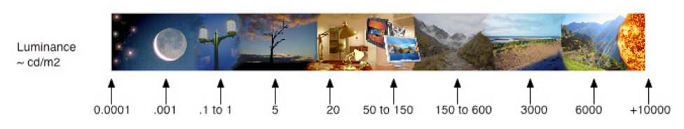
\includegraphics[width=\linewidth]{images/luminancerange}
 	\caption{نمونه‌ای از دامنه‌های روشنایی متفاوت}\label{fig:logtonemap}
 	\endminipage\hfill
 \end{figure}
 


 در این پروژه سعی شده‌است دو  روش  مهم و نسبتا پیچیده برای ارائه‌ی تصویر با دامنه‌ی دینامیکی بالا پیاده‌سازی و مقایسه شوند.
 
 در بخش اول، کلیات این علم و تعریف‌های موجود بررسی می‌شوند. در بخش دوم، تعدادی از الگوریتم‌های پیشین، پیچیدگی و نتایج آنها به اختصار مورد بررسی قرار می گیرند. دربخش سوم، دو روش  مورد نظر در این پروژه توضیح داده می‌شوند، روش پیاده‌سازی آنها شرح داده‌شده، ونتایج بررسی می شوند.
 
 \section{  نگاشت سراسری و نگاشت محلی}
 
نگاشت های سراسری، شامل نگاشت‌هایی است که با توجه به متغیرهای سراسری عکس، مانند میانگین روشنایی انجام می‌شوند. در واقع پس از محاسبه‌ی متغیرهای مطلوب از یک عکس خاص، یک تابع مشخص روی تمام پیکسل‌های عکس اعمال می‌شود. این نوع نگاشت بسیار سریع است. چون معمولا محاسبات پیچیده‌ای ندارند و همچنین می‌توانند با استفاده از
 \متن‌لاتین{look up table  }
ها انجام شوند.

مشکل این نوع نگاشت این است که به دلیل کم کردن تضاد روشنایی باعث از بین رفتن جزئیات یا تغییر رنگ ها می‌شود.

نگاشت‌های محلی، شامل نگاشت هایی است که عملکرد آن روی هر پیکسل، با توجه به متغیرهای احاطه گر آن، متفاوت است.به زبان دیگر پارامترهای تابع، در هر قسمت از تصویر، با توجه به ویژگی‌های آن قسمت از تصویر متفاوت است.

این نوع نگاشت‌ها معمولا دارای محاسبات پیچیده تری هستند، ممکن است هاله‌های مصنوعی ایجاد کنند، و تصویر را کمی تصنعی کنند. اما اگر به درستی اعمال شوند، می‌توانند بهترین تصویر ممکن را ارائه دهند.زیرا سیتستم بینایی انسان به تضادهای روشنایی محلی بیشتر حساس است تا تضادهای سراسری.


\section{تعریف روشنایی در تصاویر رنگی}

روشنایی فضا، روشنایی فیزیکی است و در واقع به معنی شدت انرژی نور است که بر حسب $cd/m^{2}$ قابل اندازه‌گیری است. در تصویر، این روشنایی به صورت مقدار $L$ در فضای  $LUV$ یا به صورت یک ترکیب خطی از کانال‌های رنگ سبز و قرمز و آبی در فضای $RGB$ تعریف می‌شود.

ضرایب این ترکیب خطی به روش‌های گوناگونی قابل تعریف است.  و ممکن است طبق دو تعریف متفاوت، ترتیب روشنایی یک محموعه  تصویر تغییر کند. تفاوت های جزئی  اهمیتی ندارند، چون تعریف دقیق و صحیحی از روشنایی وجود ندارد و این تعریف ها هر چقدر به ذهنیت ما از روشنایی نزدیک تر باشند، بهتر  هستند.

یکی از تعریف‌های متداول به صورت زیر است.

\begin{equation}
luminance = 0.27 red + 0.67 green + 0.06 blue
\end{equation}